\documentclass[12pt,a4paper^, twocolumn]{article}
\usepackage[utf8x]{inputenc}
\usepackage{amssymb}
\usepackage{amsmath}
\usepackage{hyperref}
\usepackage[ngerman]{babel}
\usepackage[noheadfoot,top=1.0cm,bottom=1.0cm,left=1.5cm,right=1.5cm]{geometry}
\usepackage{fancyhdr}
\usepackage{wasysym} % \smiley :)
\usepackage{scalefnt}
\usepackage{graphicx} % scalebox, rotatebox


%%% AND: \wedge; OR: \vee
%%% neue befehle -- bitte benutzen ;-)

\newcommand{\basis}{\mathfrak} % basis in frakturschrift
\newcommand{\menge}{\mathbb} % menge in mengenschrift ^^
\newcommand{\und}{\wedge} % logisches und
\newcommand{\oder}{\vee} % logisches oder
\newcommand{\entspr}{\widehat{=}} % entspricht zeichen
\newcommand{\liminfty}[1]{\lim \limits_{#1 \rightarrow \infty}} % lim {#1} --> infty
\renewcommand{\epsilon}{\varepsilon} % *das* epsilon!
\renewcommand{\phi}{\varphi} % *das* phi!
\newcommand{\pivot}{{\fboxsep1pt \fbox{$\ast$}}} % pivot-element in stufen-matrix
\renewcommand{\d}{\mathrm{d}} % d/dx schreiben als \frac{\d}{\d x}
\newcommand{\R}{\mathbb{R}}
\newcommand{\N}{\mathbb{N}}
\newcommand{\C}{\mathbb{C}}
\newcommand{\I}{\mathbb{I}}


%%% neue befehle -- bitte benutzen ;-)
\makeatletter
\renewcommand*\env@matrix[1][*\c@MaxMatrixCols c]{%
  \hskip -\arraycolsep
  \let\@ifnextchar\new@ifnextchar
  \array{#1}}
\makeatother

\makeatletter
\renewcommand{\section}{\@startsection{section}{1}{0mm}%
                                {-1ex plus -.5ex minus -.2ex}%
                                {0.5ex plus .2ex}%x
                                {\normalfont\large\bfseries}}
\renewcommand{\subsection}{\@startsection{subsection}{2}{0mm}%
                                {-1explus -.5ex minus -.2ex}%
                                {0.5ex plus .2ex}%
                                {\normalfont\normalsize\bfseries}}
\renewcommand{\subsubsection}{\@startsection{subsubsection}{3}{0mm}%
                                {-1ex plus -.5ex minus -.2ex}%
                                {1ex plus .2ex}%
                                {\normalfont\small\bfseries}}
\makeatother 

\parindent 0mm % Absatzeinzug auf 0 setzen
\lhead{} % Überschrift
\rhead{} % seitenzahl ausblenden -- erst nach TOC anzeigen
\cfoot{} % seitenzahl ausblenden
\renewcommand{\headrulewidth}{0mm} % header trennlinie ausblenden

\begin{document}
\scalefont{0.8} % schriftgröße skalieren: 10pt --> 8pt

\begin{center}
  {\large Analysis Merkblatt}\\
  {}
\end{center}

\section{Zahlensysteme}
	\subsection{Axiomatische Charakterisierung der Reellen Zahlen}
		$(\R, +, \cdot) $ ist ein angeordneter Körper, der die Supremumseigenschaft besitzt.
		\subsubsection{Satz}
			Es gibt nur einen einzigen angeordneten Körper, der die Supremumseigenschaft besitzt 
			(bis auf Umbenennung der Elemente).
	\subsection{Komplexe Zahlen}
		$z_1 = (a,b), z_2 = (c, d)$\\
		$z_1 z_2 = (ac - bd, ad + bc), \frac{z_1}{z_2} = 
			(\frac{ac+bd}{c^2+d^2}, \frac{cb-ad}{c^2+d^2})$ für $c^2+d^2 \neq 0$
%	\subsection{Einige nützliche Bezeichungen}
	\subsection{Rechenregeln für Suprema}
		Es seien $ X, Y \subset \R $ mit $\sup X, \sup Y \in \R $ und $ \lambda \in \R$. 
		Dann gilt:
		\begin{itemize}
			\item $\sup (X+Y) = \sup X + \sup Y $
			\item $\lambda > 0 \Rightarrow \sup(\lambda X) = \lambda \sup X $
			\item $X, Y \subset [0, \infty) \Rightarrow \sup (XY) = \sup X \cdot \sup Y$
			\item $X \subset Y \Rightarrow \sup X \leq \sup Y $
		\end{itemize}
%	\subsection{Archimedizität der Reellen Zahlen}
%	\subsection{Dichtheit der Rationalen Zahlen}
%	\subsection{Dezimaldarstellung}

\section{Ungleichungen}
\subsection{Elementare Ungleichungen}
Dreiecksungleichung: \\
$|a+b| \leq |a|+|b|$ \\
Umgekehrte Dreiecksungleichung: \\
$|a+b| \geq ||a|-|b||$ \\
Ungleichheit für geometrische Summen:\\
$1+x+x^2+x^3+\dots+x^n \leq \frac{1}{1-x} \quad (n \in \menge{N}_0, 0 \leq x < 1)$ \\
Bernoulli'sche Ungleichung:\\
$(1+x)^n \geq 1+nx \quad (n \in \menge{N}_0, x > -1)$ \\
Ungleichung zwischen geometrischem und arithmetischem Mittel: \\
$\sqrt{ab} \leq \frac{a+b}{2} \quad (a,b \geq 0)$ \\
Ungleichung vom mittleren Verhältnis:\\
	$
	\min(\frac{a_1}{b_1}, \dots, \frac{a_n}{b_n}) 
	\leq \frac{a_1+\dots+a_n}{b_1+\dots+b_n} 
	\leq \max(\frac{a_1}{b_1}, \dots, \frac{a_n}{b_n})
	\quad (b_1,\dots,b_n > 0)
	$
\subsection{Cauchy-Schwarz'sche Ungleichung}
$\sum\limits_{k=1}^n x_ky_k \leq \sqrt{\sum\limits_{k=1}^n x_k^2} \cdot \sqrt{\sum\limits_{k=1}^n y_k^2} \quad (x_1,\dots,x_n,y_1,\dots,y_n \in \menge{R})$ \\
oder auch: $\langle x,y \rangle \leq ||x|| \cdot ||y|| \quad (x,y \in \menge{R}^n)$
\subsection{Euklidische Norm}
$||x|| := \sqrt{\langle x,x \rangle} = \sqrt{\sum\limits_{k=1}^n x_k^2}$ \quad f"ur $x \in \menge{R}^n$
\subsubsection{Euklidisches Skalarprodukt}
$\langle x,y \rangle := \sum\limits_{k=1}^n x_k \cdot y_k$ \quad f"ur $x,y \in \menge{R}^n$ \\
andere Normen

\section{Folgen}
\subsection{Konvergenz von Folgen}
	Die Folge $(a_n)$ konvergiert gegen den Grenzwert $a \in \R$, falls für
	jede Genauigkeit $\epsilon > 0$ die Abschätzung $|a_n - a| \leq \epsilon$ für fast
	alle $n \in \N$ eingehalten wird.
\subsubsection{Monotonie der Grenzwertbildung}
	Es seien $a_n \to a$ und $b_n \to b$.\\
	Gilt $a_n \leq b_n \, \forall n \geq n_0 \in \N$, dann gilt $ a \leq b$.
\subsubsection{Einschließungsregel}
	Es sei $\forall \, n \geq n_0 \in \N : \, a_n \leq a_n' \leq a_n''$.
	Dann gilt 
	$$\lim_{n \to \infty} a_n = \lim_{n \to \infty} a_n'' = a 
	\qquad \Rightarrow  \qquad \lim_{n \to \infty} a_n' = a$$
\subsubsection{Konvergenz in $\R^d$ und $\mathbb{C}$}
	Die vektorwertige Folge\\
	$\N \ni n \mapsto x_n = 
		\begin{pmatrix}
			x_{n_1}\\
			\vdots \\
			x_{n_d}
		\end{pmatrix}$
	konvergiert gegen den Grenzwert $
		x = \begin{pmatrix}
			x_{1}\\
			\vdots \\
			x_{d}
		\end{pmatrix}$\\
	$$\Leftrightarrow 
		\lim_{n \to \infty} x_{n_k} = x_k 
		\quad \forall k \in \{1, \dots, d \} 
		\text{(komponentenweise Grenzwerte existieren)}$$
	Analog in $\mathbb{C}$ (isomorph zu $\R^2$).
\subsection{Beschränktheit konvergenter Folgen}
	Eine konvergente Folge $(a_n) \subset \R$ ist beschränkt.\\
	D.h. $\exists c > 0 $ mit $|a_n| \leq c \forall n \in \N$.\\
	Das gleiche gilt für Folgen aus  $\R^d$ und $\mathbb{C}$ mit $||\cdot||_2$
	bzw. dem Absolutbetrag in $\mathbb{C}$.
\subsection{Stetigkeit: Rechnen mit Grenzwerten}
	Eine Funktion $f : D \subseteq \R^d \to \R^q$ heißt 
	im Punkt $x \in D$ ihres Definitionsbereichs stetig, falls für jede Folge 
	$(x_n)$ aus $D$ gilt:
	$$
		x_n \overset{n \to \infty}{\to} x
		\qquad \Rightarrow \qquad
		f(x_n) \overset{n \to \infty}{\to} f(x)
	$$
	\subsubsection{Elementare stetige Funktionen}
	\begin{center}
	\newcommand{\infowidth}{2cm}
	\newcommand{\aufsichtwidth}{10cm}
	\begin{tabular}{|c|c|}
	\hline
	$D \subseteq \R$ &  $f(x) \in \R$ \\
	\hline
	$\R$ & $f(x) = c, c \in \R$\\
	$\R$ & $f(x) = |x|$\\
	$[0, \infty)$& $f(x) = \sqrt{x}$\\
	\hline
	$D \subseteq \R^2$ &  $f(x, y) \in \R$ \\
	\hline
	$\R^2$ & $f(x, y) = x+y$\\
	$\R^2$ & $f(x, y) = x \cdot y$\\
	$\R \times (\R \setminus \{0\}) $ & $f(x, y) = x \div y$\\
	\hline
	\end{tabular}
	\end{center}
	Summe, Produkt, Quotient zweier konvergenter Folgen ist konvergent. Für
	divergente/uneigentlich konvergente Folgen gilt das nicht.\\
	\\
	\begin{itemize}
	\item Polynome (in $\mathbb{C}$ und $\R$) sind stetig auf ganz $\mathbb{C}$ 
	bzw. $\R$.
	\item $\max(a,b) = \frac{a + b + |a-b|}{2}$ und $\min(a,b) = \frac{a+b - |a-b|}{2}$ 
	sind stetig auf $\R^2$, bzw. die entsprechenden Funktionen auch in 
	höherdimensionalen Räumen.
	\item Als Konsequenz sind auch Normen stetig.
	\end{itemize}
	
	
	\subsubsection{Stetigkeit der Verknüpfung von Funktionen}
		Sei $f : D \subseteq \R^d \to \R^q$, 
		$g : E \subseteq \R^q \to \R^p$ mit 
		$f(D) \subseteq E$ und \\
		$g \circ f : D \subseteq \R^d \to \R^p, 
		(g \circ f)(x) := g(f(x))$ die Verkfüpfung von $f$ mit $g$. 
		Dann gilt: Wenn $f$ stetig in $x \in D$ und $g$ stetig $f(x) \in E$\\
		$\Rightarrow g \circ f$ stetig in $x \in D$
\subsection{Monotone Folgen}
	$(a_n)_{n \in \N}$ monoton wachsend $\Leftrightarrow a_n \leq a_{n+1} 
	\, \forall n \in \N$\\
	$(a_n)_{n \in \N}$ monoton fallend $\Leftrightarrow a_n \geq a_{n+1} 
	\, \forall n \in \N$\\
	Strenge Monotonie gilt, falls statt $\leq, \geq$ echte Ungleichheit gilt.\\
	\subsubsection{Satz}
		Jede beschränkte, monotone Folge $(a_n)_{n \in \N} \subset \R$
		ist konvergent.
		Jede unbeschränkte, monotone Folge $(a_n)  \subset \R$ konvergiert 
		uneigentlich.
\subsection{Beschränkte Folgen}
	\subsubsection{Teilfolgen und Häufungswerte}
		Ist $(a_n) \subset \R^d$ eine beliebige Folge und 
		$(n_k)_{k \in \N} \subset \N $ 
		streng monoton wachsend, dann heißt $ (a_{n_k})_{k \in \N}$
		\textbf{Teilfolge} von $(a_n)$.\\
		Grenzwerte konvergenter Teilfolgen heißen \textbf{Häufungswerte}. Der maximale
		bzw. minimale Häufungswert werden als $\limsup$ bzw. $\liminf$ 
		bezeichnet und wie folgt definiert:
		$$ 
		\limsup_{n \to \infty} a_n := 
		\lim_{n \to \infty} \left( \sup_{k \geq n} a_k \right) ,
		\qquad \quad
		\liminf_{n \to \infty} a_n := 
		\lim_{n \to \infty} \left( \inf_{k \geq n} a_k \right)
		$$
	\subsubsection{Satz von Bolzano-Weierstrass}
		Jede beschränkte Folge $(a_n)_{n \in \N} \subset \R$ besitzt
		mindestens eine konvergente Teilfolge $(a_{n_k})_{k \in \N}$ (also min.
		einen Häufungswert).
	\subsubsection{Lemma Seite 6/14, VL 6}
		Sei $(a_n)$ beschränkt. Dann gilt: \\
		$$ \limsup_{n \to \infty} a_n = \liminf_{n \to \infty} a_n = a
		\qquad \Leftrightarrow \qquad
		\lim_{n \to \infty} a_n = a$$
	\subsubsection{Korollar Seite 7/14, VL 6}
		Jede beschränkte Folge $(a_n)_{n \in \N} \subset \R^d$ besitzt
		mindestens eine konvergente Teilfolge.\\
		$(a_n)$ ist genau dann konvergent, wenn sie genau einen Häufungswert besitzt.	
	\subsection{Exponentialfunktion}
		$e^x = \lim_{n \to \infty} \left(1 + \frac{x}{n} \right)^n, x \in \R$\\
		$e^{\frac{x+y}{2}} = e^{\frac{x}{2}} \cdot e^{\frac{y}{2}} = \sqrt{e^xe^y}$
	\subsubsection{Abschätzungen der Exponentialfunktion}
		$e^x \geq 1 + x \forall x \in \R$\\
		$e^{-x} \geq 1 - x \qquad \Rightarrow \qquad e^x \leq \frac{1}{1-x}$ für $x < 1$ 
		

\section{Reihen}
	Sei $(a_n) \subset \C$. Die Folge $(s_n)$ mit 
	$s_n := a_1 + a_2 + \dots + a_n = \sum\limits_{k=1}^{n} a_k$ heißt (unendliche) Reihe
	(Schreibweise $\sum a_k$) mit den Reihengliedern $a_n$ und den \textbf{Partialsummen}
	$s_n$.
	\subsection{Konvergenz von Reihen}
		Die Reihe $(s_n)$ heißt konvergent, wenn $s_n \to s \in \C$
		(Schreibweise: $s = \sum\limits_{k=1}^{\infty} a_k = a_1 + a_2 + \dots$). 
		$s$ heißt Summe oder Wert der Reihe $(s_n)$.
		Wenn $s_n \to \pm \infty$, schreiben wir auch 
		$\sum\limits_{k=1}^{\infty} a_k = \pm \infty$.\\
		\subsubsection{Notwendige Bedingung für Konvergenz}
			$\sum\limits_{k=1}^{\infty} a_k = s 
			\qquad \Rightarrow \qquad 
			a_k \to 0 (n \to \infty)$
		\subsubsection{Reihen mit nichtnegativen Gliedern}
			$(s_n)$ mit $s_n = \sum\limits_{k=1}^{n} a_k$ mit $a_k \geq 0$ konvergiert 
			($\sum\limits_{k=1}^{\infty} a_k < \infty$) $\Leftrightarrow (s_n) $ beschränkt.
		\subsubsection{Beispiele}
			\begin{itemize}
				\item Teleskopreihe: $ \sum\limits_{k=1}^{\infty} \frac{1}{k(k+1)}  = 1$
				\item Geometrische Reihe: $ \sum\limits_{k=1}^{\infty} z^k = \frac{1}{1-z},
				\qquad z \in \C, |z| < 1 $
				\item Harmonische Reihe: $\sum\limits_{k=1}^{\infty} \frac{1}{k} = \infty $
				\item $\sum\limits_{k=1}^{\infty} \frac{1}{k^2}$ konvergiert nach 
				Majoratenkriterium.
			\end{itemize}

	\subsection{Konvergenzkriterien}
		\subsubsection{Majorantenkriterium}
			Seien $( \sum\limits_{k=1}^n a_k) \in \C$ und 
			$( \sum\limits_{k=1}^n b_k) \in \R$ Reihen mit $|a_k| \leq b_k$.\\
			$( \sum\limits_{k=1}^n b_k)$ heißt Majorante von 
			$( \sum\limits_{k=1}^n a_k)$ und es gilt:
			\begin{itemize}
				\item $( \sum\limits_{k=1}^n b_k)$ konvergiert 
				$\Rightarrow ( \sum\limits_{k=1}^n a_k)$ konvergiert
				\item $( \sum\limits_{k=1}^n a_k)$ divergiert 
				$\Rightarrow ( \sum\limits_{k=1}^n b_k)$ divergiert
				\item $\left| \sum\limits_{k=1}^{\infty} a_k \right|
					\quad \leq \quad \sum\limits_{k=1}^{\infty} |a_k| 
					\quad \leq \quad \sum\limits_{k=1}^{\infty} b_k$
			\end{itemize}
		\subsubsection{Quotientenkriterium}
			$( \sum\limits_{k=1}^n a_k) \in \C$ und $a_k \neq 0 \quad \forall k \leq k_0$
			mit Grenzwert $ q:= \lim_{k \to \infty} |\frac{a_{k+1}}{a_k}|$
			\begin{itemize}
			\item $q < 1 \Rightarrow ( \sum\limits_{k=1}^n a_k)$ konvergiert
			\item $q > 1 \Rightarrow ( \sum\limits_{k=1}^n a_k)$ divergiert
			\item $q = 1 \Rightarrow $ keine Aussage möglich 
			\end{itemize}
		\subsubsection{Wurzelkriterium}
			$(\sum\limits_{k=1}^n a_k)$ mit 
			$\rho := \limsup_{k \to \infty} \sqrt[k]{|a_n|} $
			\begin{itemize}
				\item $\rho < 1 \Rightarrow ( \sum\limits_{k=1}^n a_k)$ konvergiert
				\item $\rho > 1 \Rightarrow ( \sum\limits_{k=1}^n a_k)$ divergiert
				\item $\rho = 1 \Rightarrow $ keine Aussage möglich 
			\end{itemize}
		\subsubsection{Leibnizsches Konvergenzkriterium}
			$(a_n) \in \R$ und $(a_n)$ ist eine \textit{monoton fallende Nullfolge}\\
			$ \Rightarrow \sum\limits_{k=0}^ \infty (-1)^k a_k = s \quad$ konvergiert.
		\subsubsection{Praktische Tipps zur Untersuchung der Konvergenz}
			\begin{enumerate}
			\item Bekannte Beispiele kennen
			\item Untersuche, ob es sich bei $a_n$ um eine Nullfolge handelt.
			\item Betrachte $\sum |a_k|$ und vergleiche mit bekannten Reihen. 
				Findet Majorantenkriterium Anwendung?
			\item Wende Quotientenkriterium an
			\item Wende Wurzelkriterium an
			\item Alternierende Reihe? 
			\end{enumerate}

	\subsection{Reihenumordnung}
		\subsubsection{Absolute Konvergenz}
			Sei $(a_n) \subset \C$.
			Man sagt $\sum\limits_{k=1}^{n} a_k$ konvergiert absolut, wenn 
			$\sum\limits_{k=1}^{n} |a_k| < \infty$. Konvergiert $\sum a_k$ absolut, so 
			konvergiert $\sum a_k$ nach Majorantenkriterium.
		\subsubsection{Umordnungssatz}
			Nur absolut konvergente Reihen können beliebig umgeordnet werden, ohne dass
			sich ihre Summe ändert.
%		\subsubsection{Multiplikation von Reihen}
			
		
\section{Konsequenzen der Stetigkeit}
	\subsection{Zwischenwertsatz} 
		Eine \textit{stetige} Funktion $f: [a, b] \to \R$ nimmt jeden Wert $y^*$ zwischen
		$f(a)$ und $f(b)$ an mindestens einer Stelle $x^* \in [a,b]$ an.\\
		D.h. $\exists x^* \in [a,b]: f(x^*) = y^*$.\\
		Sei $f$ streng monoton. Dann ist $x^*$ eindeutig.
	\subsection{Satz: Stetige Umkehrfunktion}
		Eine stetige, streng monotone Funktion $f: [a, b] \to \R$ besitzt eine
		Umkehrabbildung $f^{-1} : [f(a), f(b)] \to \R$ mit $f^{-1}(y) = x$ für $f(x) = y$,
		die ebenfalls stetig und streng monoton ist.
	\subsection{Existenz von Maximum und Minimum}
	$K \neq \emptyset$ aus $\R$ kompakt (abgeschlossen \& beschränkt) besitzt Max und Min.\\
	$K$ Kompakt, $f$ stetig $\Rightarrow f(K) $ kompakt.\\
	Jede \emph{stetige} Funktion $f: K \in \R^d$ mit Definitionsbereich $\emptyset \neq K$
	\emph{kompakt} nimmt ihr Maximum und Minimum an.\\

	$K$ kompakt $ \Leftrightarrow $ Jede Folge aus $K$ besitzt eine Konvergente Teilfolge mit Häufungswert (HW) \underline{in $K$}



\section{Ableiten}
	Def.: $\I \in \R$ Intervall, $f: \I \to \R$ \\
	$f$ heißt differenzierbar in $x_0 \in \I \\
	\Leftrightarrow \lim\limits_{x \to x_0} \frac{f(x) - f(x_0)}{x - x_0} = c \in \R \\
	\Leftrightarrow \forall (x_n)_{n \in \N} \subset \I$ mit $x_n \to x_0$ folgt, dass $\frac{f(x_n) - f(x_0)}{x_n-x_0} = c \in \R
	\Leftrightarrow \lim\limits_{n \to 0} \frac{f(x_0 + h)-f(x_0)}{h} = \in \R$ \\
	Falls der Grenzwert 
	$\Leftrightarrow \lim\limits_{x \to x_0} \frac{f(x) - f(x_0)}{x - x_0}$ existiert,
	schreiben wir $f'(x_0) = \lim\limits_{x \to x_0} \frac{f(x) - f(x_0)}{x - x_0}$
	\begin{itemize}
	\item $f$ diffbar in $x_0 \Rightarrow f$ stetig in $x_0$
	\item Kettenregel: $f,g$ Funktionen mit $f$ diffbar in $g(x_0), g$ diffbar in $x_0$
		$\Rightarrow (f \circ g)'(x_0) = f'(g(x_0))g'(x_0)$
	\item $f: \I \to \R, f$ injektiv $(f(x) = f(y) \Rightarrow x=y) \rightarrow f:\I \to f(\I) bijektiv \Rightarrow f^{-1}$ existiert. \\
		Ist $f'(y) \neq 0 \Rightarrow (f^{-1})'(x) = \frac{1}{f'(f^{-1}(x))}$
	\item Arithmetikregeln:
		\begin{itemize}
		\item $(f + \lambda g)' = f' + \lambda g'$
		\item $(f \cdot g)' = (f' \cdot g) + (f \cdot g')$
		\item $(\frac{f}{g})' = \frac{f'\cdot g - f \cdot g'}{g^2}$
		\end{itemize}
	\end{itemize}


\subsection{Anwendung der Ableitungen}
	$f:[a,b] \to \I$ hat bei $x_0 \in [a,b]$ ein
	\begin{itemize}
	\item glob Max $\Leftrightarrow f(x) = f(x_0) \quad \forall x \in [a,b]$
	\item lok Max $\Leftrightarrow \exists \epsilon >0: \forall x \in (x_0-\epsilon, x_0+\epsilon) \cap [a,b]: f(x) \leq f(x_0)$
	\end{itemize}
	Notwendige Bedingung f"ur lokale Maxima: \\
	$f[a,b] \to \R ($diffbar in $x_0)$, ist $x_0 \in (a,b)$ lok Extremum $\Rightarrow f'(x_0) = 0$ \\
	Hinreichende Bedingung: \\
	$f: (a,b) \to \R \ 2 \times$ diffbar in $x_0 \in (a,b)$ mit $f'(x_0) = 0$
	\begin{itemize}
	\item $f''(x_0) < 0 \Rightarrow f$ lokales Maximum in $x_0$
	\item $f''(x_0) > 0 \Rightarrow f$ lokales Minimum in $x_0$
	\item $f''(x_0) = 0 \Rightarrow$ keine Aussage direkt möglich.
	\end{itemize}

\subsection{Mittelwertsatz der Differentialrechnung}
	Sei $f : [a, b] \to \R$ stetig und diffbar. Dann:
	$$
		\exists \xi \in (a, b) : \frac{f(b)-f(a)}{b-a} = f'(\xi)
	$$
	Allgemeiner mit $g:[a,b] \to \R, \quad g'(x) \neq 0 \, \forall \, x \in [a,b]$:
	$$
		\exists \xi \in (a, b) : \frac{f(b)-f(a)}{g(b)-g(a)} = \frac{f'(\xi)}{g'(\xi)}
	$$

\subsection{Regel von L'Hospital}
	$f,g: (a,b) \to \R$ diffbar, $a,b \in \R \cup \{\pm \infty\}$ \\
	Sei $x_0 \in (a,b)$ und gilt \\
	entweder $f(x), g(x) \to \infty$ f"ur $x \to x_0$  \\
	oder $f(x),g(x) \to 0$ f"ur $x \to x_0$ \\
	$ \Rightarrow \lim\limits_{x \to x_0} \frac{f(x)}{g(x)} = \lim\limits_{x \to x_0} \frac{f'(x)}{g'(x)} \in \R$

\subsection{Konvexit"at}
	Mengen: $D \in \R^n$ ist konvex $\Leftrightarrow \forall x,y \in D \ [x,y] \in D$ \\ 
	$[ x, y ] = \{\lambda x + (1- \lambda)y | \lambda \in [0,1] \}$ \\
	Funktionen: $D \subseteq \R^n$ konvex \\
	$f: D \to \R$ konvex 	$\Leftrightarrow f(\lambda x + (1-\lambda)y) \leq \lambda f(x) + (1 - \lambda ) f(y)$\\
	$f(a,b) \to \R \ 2 \times$ stetig diffbar.  $f$ konvex $\Leftrightarrow f''(x) \geq 0$

\subsection{Mehrdimensionales Ableiten}
	Def.: $U \in \menge{R}^n$ offen, \quad $f:U \to \menge{R}^m$ \\
	$f$ heißt diffbar in $x \in U \Leftrightarrow \exists$ lin. Abb. $A: U \to \menge{R}^m \quad A \in \menge{R}^{m \times n}$ mit
	$f(x+h) = f(x) + A(x)h + o(||h||) \rightarrow f(x+h) = f(x) + A(x)h$ \\
	$A$ ist durch $f$ eindeutig bestimmt aber abh"angig von $x$.\\ $A$ heißt Jakobimatrix. $A(x) := J_f(x) =: Df(x)$
	\begin{itemize}
	\item $m,n$ beliebig: $A(x) = \begin{pmatrix}
			\frac{\partial f_1}{\partial x_1} 	& \cdots 	& \frac{\partial f_1}{\partial x_n} \\
			\vdots					& \ddots	& \vdots	\\
			\frac{\partial f_m}{\partial x_1}	& \cdots	& \frac{\partial f_m}{\partial x_n}
		\end{pmatrix} = \begin{pmatrix}
			(\nabla f_1)^T \\
			\vdots \\
			(\nabla f_m)^T
		\end{pmatrix}$
	\item $m = 1, n \in \menge{N}$ \\
		$A(x) = (\nabla f(x))^T = \left ( \frac{\partial f}{\partial_1}, \cdots, \frac{\partial f}{\partial_n} \right )$ \\
		Falls $f$ stetig partiell diffbar ist $\Rightarrow f$ ist diffbar. \\
		$D^2 f(x) = \begin{pmatrix}
			\frac{\partial^2 f}{\partial x_1 \partial x_1} 	& \cdots	& \frac{\partial^2 f}{\partial x_1 \partial x_n} \\
			\vdots						& \ddots	& \vdots	\\
			\frac{\partial^2 f}{\partial x_n \partial x_1} 	& \cdots	& \frac{\partial^2 f}{\partial x_n \partial x_n}
		\end{pmatrix}$ \\
		$D^2 f = H_f$ ist eine symmetrische $n \times n$-Matrix und heißt Hesse-Matrix.
	\end{itemize}




\section{Integral}
Defs.:  \dots \\
Falls $f:[a,b] \rightarrow \menge{R}$ beschr"ankt und monoton oder $f$ st"uckweise stetig, dann ist $f$ Riemann integrierbar.
\underline{Hauptsatz der Differential und Integralrechnung} \\
	Sei $f:[a,b] \rightarrow \menge{R} \textit{ stetig }, c \in [a,b]$ fest, dann $\quad F(x) := \int\limits_c^x f(y) \d y$
	\begin{enumerate}
	\item stetig diffbar
	\item $F'(x) = f(x) \quad \forall x \in [a,b]$
	\item $\int\limits_a^b f(x) \d x = F(b) - F(a)$
	\end{enumerate}
\subsection{Partielle Integration}
	$\int\limits_a^b f \cdot g' \d x = f \cdot g \big|_a^b - \int\limits_a^b f' \cdot g \ \d x$ oder $ \int u \d v = uv - \int v \d u$
\subsection{Substitution}
	$g:[a,b] \rightarrow \menge{R}, F: g([a,b]) \rightarrow \menge{R}$ stetig diffbar, $F' = f$ \\
	$\int\limits_a^b f(y) \d y = \int\limits_{g^{-1}(a)}^{g^{-1}(b)} f(g(x)) g'(x) \d x$ \\
	$x = g^{-1}(y) \Leftrightarrow y=g(x) \quad \frac{\d y}{\d x} = g'(x)$
\subsection{Uneigentliche Integrale}
	Sei $f:[a,b] \rightarrow \menge{R}$ integrierbar $\forall [\alpha, \beta], a \leq \alpha < \beta < b$ \\
	$ \Rightarrow \int\limits_a^b f(x) \d x = \lim\limits_{\beta \to b} \int\limits_a^\beta f(x) \d x$
\subsection{Integralkriterium}
	F"ur $f: [1,\infty) \to [0, \infty )$ monoton fallend gilt: \\
	$0 \leq \lim\limits_{n \to \infty} ( \underbrace{\sum\limits_{k=1}^n f(k)}_{b_n} - \underbrace{\int\limits_1^{n+1} f(x) \d x}_{c_n} ) \leq f(1)$ \\
	$\Rightarrow \sum\limits_{n=1}^\infty f(n) < \infty \Leftrightarrow \int\limits_1^\infty f(x) \d x < \infty$
\subsection{Mehrdimensionale Integrale}
\subsubsection{"uber Quader $Q \in \R^n$}
	$\int\limits_Q f(x_1,\dots,x_n) \d x_1 \dots \d x_n = 
	\int\limits_{a_n}^{b_n} \dots \int\limits_{a_2}^{b_1} ( \int\limits_{a_1}^{b_1} f(x_1,\dots,x_n) \d x_1 ) \d x_2) \dots \d x_n$ \\
	kurz: $\int\limits_Q f(x) \d^n x$ oder $\int\limits_Q f(x) \d x$ \\
	Tr"ager von f: $Supp(f) = \overline{\{x \in \R^n : f(x) \neq 0\}}$ Im Folgende seien die Tr"ager aller Funktionen kompakt. \\
	Charakteristische Funktion $\chi_K$ einer kompakten Menge $K \subset \R^n:
	X_K(x) = \begin{cases}1, \text{  falls } x \in K \\ 0,  \text{   falls } x \in \R^n \setminus K.\end{cases}$ \\
	Volumen von $K$:  $Vol(K) := \int\limits_{\R^n} \chi_K(x) \d^n x \quad \in \R_+  \entspr \quad \int\limits_K 1 \ \d^n x$
\subsubsection{"uber beliebige stetige Funktionen mit kompakten Tr"ager}
	Sei $ \in \R^{n \times n}$ invertierbar: $A\int\limits_{\R^n} f(Ax) |det A| d^n x = \int\limits_{\R^n} f(y) d^n y$ \\
	Transformationssatz: Seien $U,V \subset \R^n$ offene Mengen und $\phi: U \to V$ stetig diffbar mit $\phi^{-1} : V \to U$ stetig diffbar.
	Dann gilt f"ur alle stetigen Funktionen f mit kompaktem Tr"ager in V: \\
	$\int\limits_U f(\phi(x)) \cdot \big| \det D \phi(x) \big| d^nx = \int\limits_V f(y) d^n y$


\section{Potenzreihe}
	Sei $(a_n)_{n\in \menge{N}}$ Folge, 
	dann heißt $f:(-r,+r) \rightarrow \menge{R} \quad f(x) = \sum\limits_{k=0}^\infty a_kx^k$ Potenzreihe. \\
	$r > 0$ heißt Konvergenzradius, $r = \frac{1}{\limsup \sqrt[n]{|a_n|}}$. \\
	Welche Funktionen $f$ haben die Darstellung $f(x) = \sum\limits_{k=0}^\infty a_kx^k \quad \forall x \in (-r,r) \rightarrow$ \underline{Taylorentwicklung} \\
	$f: \menge{I} \rightarrow \menge{R}, \menge{I} = (a,b) \quad f (n+1)$-mal stetig diffbar, dann: \\
	$\forall x,a \in \menge{I}: (x) = \underbrace{ \sum\limits_{k=0}^{n} \frac{f^{(k)} (a)}{k!}(x-a)^k }_{\text{Taylorpolynom n-ten Grades von f um a}} + R_{n+1}(a,x)$ \\
	$R_{n+1}(a,x) = \begin{cases}
		\frac{1}{n!} \int\limits_a^x(x-t)^nf^{(n+1)}(t) \d t \\
		\frac{f^{(n+1)}(\xi)}{(n+1)!} (x-a)^{n+1} \quad \xi \in [x,a]
	\end{cases}$ \\
	falls f $\infty$-mal diffbar, $R_{n+1}(x) \rightarrow 0 (n \rightarrow \infty)
	\Rightarrow f(x) = \sum\limits_{k=0}^\infty \frac{f^{(k)}(a)}{k!} (x-a)^k$ \quad (Taylorreihe von f um a) \\
	$f:\menge{R} \rightarrow \menge{R}$ heißt analytisch in $x=0$, falls f als $f(x) = \sum\limits_{k=0}^\infty a_k x_k \quad \forall |x| < r$ darstellbar ist.
	\begin{itemize}
		\item $f \in C^\infty((-r,r))$ 
		\item $f$ analytisch, $g$ analytisch $\Rightarrow f \circ g$ analytisch mit\\
			$(f \circ g)(x) = \sum\limits_{k=0}^\infty \sum\limits_{j=0}^\infty (a_j \cdot b_{k-j})x^k \quad , |x| < \min\{r_f, r_g\}$
		\item Falls $g(0) = b_0 \neq 0$, so ist $\frac{f}{g}$ in $x=0$ analytisch und
			$(\frac{f}{g}(x) = \sum\limits_{k=0}^\infty \underbrace{\frac{1}{b_0}(a_k - \sum\limits_{j=0}^{k-1} c_jb_{k-j})}_{c_k} x^k$
		\item $a_k = \frac{f^{(k)}(0)}{k!}$
		\item $f$ analytisch, $f(0) \neq 0 \Rightarrow \frac{1}{f}$ analytisch
	\end{itemize}
\subsection{wichtige Potenzreihen}
	$e^x = \sum\limits_{k=0}^\infty \frac{x^k}{k!} \quad x \in \R$ \\
	$\sin x = \sum\limits_{k=0}^\infty (-1)^k \frac{x^{2k+1}}{(2k+1)!} \quad x \in \R$ \\
	$\cos x = \sum\limits_{k=0}^\infty (-1)^k \frac{x^{2k}}{(2k)!} \quad x \in \R$ \\
	$\ln (1+x) = \sum\limits_{k=0}^\infty (-1)^k \frac{x^{k+1}}{k+1} \quad |x| < 1$\\
	$\arctan x = \sum\limits_{k=0}^\infty \frac{(-1)^k}{2k+1} x^{2k+1} \quad |x| \leq 1$ \\
	$\frac{1}{\sqrt{1+x}} = \sum\limits_{k=0}^\infty \frac{(-1)^k}{4^k} \binom{2k}{k} x^k$



\section{Kurven}
	\begin{itemize}
	\item{Def.:} Sei $\gamma : I \rightarrow \menge{R}^n$ eine diffbare Kurve, 
		dann heißt $\gamma'(t)$ Tangentialvektor (TV) oder Geschwindigkeitsvektor von $\gamma$ zum Zeitpunkt $t$ \\
		$||\gamma'(t)|| = \sqrt{\gamma'_1(t)^2 + \dots + \gamma'_n(t)^2}$ heißt Geschwindigkeit zum Zeitpunkt t \\
		$\frac{\gamma'(t)}{||\gamma'(t)||}$ heißt Tangentialeinheitsvektor (TEV) (falls $\gamma'(t) \neq 0$).
		$\gamma: I \rightarrow \menge{R}^n$ diffbar heißt regul"ar falls $\gamma'(t) \neq 0 \quad \forall t \in I$
	\item{Satz:} Eine außer an endlich vielen Stellen stetig diffbare Kurve $\gamma: I \rightarrow \menge{R}^n, I=[a,b]$ ist rektifizierbar und hat Länge
		$S(\gamma) = \int\limits_a^b || \gamma(t) || \d t$
	\item{Korollar:} Sei $f:[a,b] \rightarrow \menge{R}$ stetig diffbar, $\gamma:[a,b] \rightarrow \menge{R}^2$ \\
		$\gamma(x) = (x, f(x))$, 
		dann $S(f) = \int\limits_a^b\sqrt{1+f'^2(x)} \d x $
	\end{itemize}


\subsection{Parameterwechsel}
	Sei $\gamma : [a,b] \rightarrow \menge{R}^n$ Kurve und rektifizierbar. \\
	Ziel: $\tilde\lambda : [a', b'] \rightarrow [a,b]$ mit gleicher Spur wie $\gamma$, aber $DG = 1 \ \forall t \in [a', b']$ \\
	\begin{enumerate}
	\item{}  Sei $\phi:[a', b'] \rightarrow [a,b]$ stetig, bijektiv, dann heißt $\phi$ Parametertransformation von $[a,b]$ nach $[a',b']$ \\
	Definiere: $\tilde\gamma = \gamma \circ \phi, \tilde\gamma:[a', b'] \rightarrow \menge{R}^n$ mit $\tilde\gamma([a',b']) = \gamma(\phi([a',b'])) = \gamma([a,b])$ \\
	\item{} $S(\xi) = \int\limits_a^\xi ||\gamma'(t)|| \d t, s(0) = 0, s(b) = S(\gamma)$ \\
	$s'(\xi) = ||\gamma'(\xi)|| > 0$ \\
	$s [a,b] \rightarrow [0, S(\gamma)]$ und $s(t) = \int\limits_0^t ||\gamma'(\tau)|| \d \tau $ \\
	$s^{-1}[0,S(\gamma)] \rightarrow [a,b] \qquad s^{-1}$ wird $\phi$ sein. \\
	$\tilde\gamma'(\xi) = (\gamma \circ s^{-1})'(\xi) = \gamma'(s^{-1}(\xi)) \cdot (s^{-1})'(\xi) = 
	\gamma'(s^{-1}(\xi)\cdot \frac{1}{s'(s^{-1}(\xi))} = \gamma'(s^{-1}(\xi) \cdot \frac{1}{||\gamma'(s^{-1}(\xi))||}$
	\end{enumerate}

\subsection{Kr"ummung}
	Sei $T(S) = \gamma'(s)$ Tangentialvektor von $\gamma$ \\
	Hat $\gamma$ konstante Geschwindigkeit 1, so ist die Kr"ummung $K$ zur Stelle $s$ definiert als: \\
	$K(s) = || \lim\limits_{\Delta s \to 0} \frac{T(s + \Delta s) - T(s)}{\Delta s} || = || T'(s) ||$ \\
	Sei $N(t) := DT(t)$, mit $D =$ "Rotation um 90°", Normaleneinheitsvektor. \\
	Ist $\gamma$ zweimal stetig diffbar mit Geschwindigkeit 1, dann ist:
	$K(s) = \langle T'(s), N(s) \rangle, \quad | K(s) | = || T'(s) ||$ \\
	Falls $\gamma = (x,y)$, gilt $K(t) = \frac{\dot{x}\ddot{y} - \dot{y}\ddot{x}}{\sqrt{\dot{x}^2 + \dot{y}^2}^3} (t)$ \\
	Falls $\gamma = (x, f(x))$ gilt $K(x) = \frac{f''(x)}{\sqrt{1+f'^2(x)}^3}$ \\
	Kr"ummungsradius $\rho (t) := \frac{1}{K(t)}$ \\
	Kr"ummungsmittelpunkt $m(t) := \gamma(t) + \rho(t)N(t)$



\section{Differentialgleichungen}
\subsection{Skalare gew"ohnliche DGL 1. Ordnung}
	lässt sich ein Anfangswertproblem schreiben als \\ $x' = f(t)g(x) \quad x(t_0) = x_0$  \\
	und sind ferner $f,g$ stetig und $g(x_0) \neq 0$, dann existiert eine lokale stetige Lösung $\phi(t)$ mit \\
	$\int\limits_{t_0}^t f(\tau) \d \tau = \int\limits_{x_0}^{\phi(t)} \frac{1}{g(\xi)} \d \xi$ \\
	Falls $g(x_o) = 0  \quad \Rightarrow \quad \phi(t) = x_0$

\subsection{Skalare lineare gew"ohnliche DGL $n$-ter Ordnung}
	$x^{(n)} + a_{n-1}x^{(n-1)} + \dots + a_0x = b(t)$ \\
	Alle Lösungen lassen sich schreiben als $\phi(t) = \phi_h(t) + \phi_s(t)$ \\
	Bestimmung der homogenen Lsg: \\
	$p(\lambda) = \lambda^n + a_{n-1}\lambda^{n-1} + \dots + a_0\lambda^0$  \\
	Seinen $\lambda_1,\dots,\lambda_s$ verschiedene Nullstellen des Polynoms $p(\lambda)$ mit den Vielfachheiten $r_1,\dots,r_s$,
	dann bilden folgende Funktionen eine Lösungsbasis $\langle \phi_h(t) \rangle$ des homogenen Problems: \\
	$e^{\lambda t}, te^{\lambda_jt},\dots,t^{r_j-1}e^{\lambda_jt} \quad ( 1 \leq j \leq s )$ \\
	Fall 1: Alle $\lambda_j$ reell $\quad \Rightarrow$ bereits reelle Lösungsbasis. \\
	Fall 2: $\lambda_k$ komplex $\Rightarrow \overline{\lambda_k}$ auch Nullstelle von $p$
		$\lambda_k = \alpha_k + i\beta_k$ und $\overline{\lambda_k}$ ersetzen durch: 
		$te^{\alpha_kt}cos(\beta_kt), t^ke^{\alpha_kt}sin{\beta_kt} \quad (1 \leq k \leq r_j-1)$

\subsection{Lineare gew"ohnliche DGL im $\menge{R}^n$}
	Sei $y = (y_1,\dots,y_n)^T \in \menge{R}^n$, dann $y' = Ay, A \in \menge{R}^{n\times n}$ Matrix \\
	Sind $y_1(t),\dots,y_n(t)$ linear unabh"angige reelle Fundamentallösungen von $y' = Ay$,
	so ist \\
	$y(t) = \alpha_1 y_1(t)+\dots+\alpha_ny_(t) \quad (\alpha_1,\dots,\alpha_n \in \menge{R}$ beliebig$)$ die allgemeine L"osung\\
	Berechnung der Fundamentall"osungen:
	\begin{enumerate}
	\item{} Sei $\lambda \in \menge{C}$ ein Eigenwert von $A$, $z \in \menge{C}^n \setminus \{0\}$ der zugeh"orige Eigenvektor,
		dann ist $y(t) = e^{\lambda t} \cdot z$ eine Lösung von $y' = Ay$  \\
		denn $y(t) = e^{\lambda t} \cdot z, Ax = Ae^{\lambda t}z = e^{\lambda t}Az = \lambda e^{\lambda t}z$ \\
		Existieren zum Eigenwert $\lambda \in \menge{C}$ linear unabh"angige Eigenvektoren $z_1,\dots,z_k$, so sind die Lösungen
		$y_1(t) = e^{\lambda t}z_1, \dots, y_k(t) = e^{\lambda t}z^k$ linear unabh"angig.
	\item{} Sei $\lambda \in \menge{C} \setminus \menge{R}$, d.h. $\lambda = \alpha + i\beta, \beta \neq 0 \quad z \in \menge{C}^n \setminus \{0\}$ sein EV,
		dann sind $y_1(t) = Re(e^{\lambda t} \cdot z), \quad y_2(t) = Im(e^{\lambda t} \cdot z)$ zwei linear unabh"angige reelle L"osungen von $y' = Ay$ 
		und $\overline\lambda$ kann ausgeschlossen werden.
	\item{} Eigenvektoren zu verschiedenen Eigenwerten sind linear unabh"angig.
	\end{enumerate}

\subsection{Satz von Picard-Lindel"of}
	Gegeben folgendes Anfangswertproblem: $y' = f(t,y) \quad y(t_0) = x_0$ \\
	Sei $\phi$ stetig und $\frac{\partial f}{\partial y'_j} \quad \forall j.1 \leq j \leq n$ stetig,
	dann hat AWP eine eindeutige L"osung in der lokalen Umgebung von $t_0$
\\\\\\


% @raphi: Hier Beispiele von den zu findenden Folgen
% TODO: erklärungen von dem spaß, und noch mehr. momentan zu müde
% Blatt 10
\section{Nützliches}
	\subsection{Beispiele für Folgen}
		$(a_n)_{n \in \N} \to 0, \, (b_n)_{n \in \N} \to +\infty$\\
		\begin{itemize}
			\item $(a_n b_n) \to 0$: 
				$ \qquad \qquad \qquad a_n := 0, \, b_n := n$
			\item $(a_n b_n) \to a \in \R \setminus \{0\}$: 
				$ \qquad a_n := \frac{a}{n}, \, b_n := n$
			\item $(a_n b_n) \to + \infty$: 
				$ \qquad \qquad a_n := \frac{1}{n}, \, b_n := n^2$
			\item $(a_n b_n) \to - \infty$: 
				$ \qquad  \qquad a_n := -\frac{1}{n}, \, b_n := n^2$
			\item $(a_n b_n)$ unbeschränkt und konvergiert nicht uneigentlich:\\
				$a_n := (-1)^n\frac{1}{n}, \, b_n := n^2$
			\item $(a_n b_n)$ beschränkt und divergiert:\\ 
				$a_n := -\frac{1}{n}, \, b_n := n$
		\end{itemize}
	\subsection{Rekursiv definierte Folgen und ihre Grenzwerte}
	Gegeben sei eine rekursiv definierte Folge $(a_n)_{n \in \N}$. 
	Zu zeigen: $(a_n)$ konvergiert und der Grenzwert ist $a$.
	\begin{enumerate}
		\item Monotonie zeigen 
		\item Beschränktheit zeigen (die ersten beiden Schritte häufig mit Induktion)
		\item Konvergenz folgern (mehr oder weniger instant aus den beiden vorherigen Punkten)
		\item Grenzwert bestimmen durch Grenzübergang in der Rekursionsrelation. Konkret heißt
		das: Auf beiden Seiten der Rekursionsrelation den $\lim\limits_{n \to \infty}$ bilden.\\
		Bsp.: $a_{n+1}^2 = 1 + a_n \quad \Rightarrow \lim\limits_{n \to \infty} a_n^2 =
		\lim\limits_{n \to \infty} (1 + a_n)
		\Rightarrow \dots $\\
		$\Rightarrow a^2 = 1 + a_n$.
	\end{enumerate}
	\subsection{Häufungswerte}
	Beispiele für \emph{divergierende} Folgen $(a_n)_{n \in \N} \in \R$:\\
	kein Häufungswert: $a_n:= n$\\
	genau einen Häufungswert:
	$$a_n := \begin{cases} 1 & n \equiv 0 \pmod{2} \\ n & \text{sonst} \end{cases} $$
	genau zwei Häufungswerte: $a_n := (-1)^n$\\
	unendlich viele Häufungswerte: $a_n := n \cdot 10^{\lfloor- \log_{10}(n+1) \rfloor}$

\subsection{Reihen}
Reihe $\sum \limits_{n=0}^\infty a_n$ mit $\limsup \limits_{n \to \infty} \sqrt[n]{|a_n|} = 1$ \\
divergiert: $ \sum \limits_{n=1}^\infty \frac{1}{n}$ \\
absolut konvergiert: $ \sum \limits_{n=1}^\infty \frac{1}{n^2}$ \\
konvergiert, nicht absolut: $\sum \limits_{n=1}^\infty \frac{(-1)^n}{n} $ oder $\sum \limits_{n=0}^\infty \frac{(-1)^n}{2n+1}$\\

\subsection{Folgen und Differenzierbarkeit}
Folge von Funktionen $f_n: [a,b] \rightarrow \R, b > a$, die punktweise gegen $f$ konvergiert:
$f_n$ stetig, aber $f$ nicht\\
$f_n(x) := x^n$ \\\\
$f_n$ stetig differenzierbar, aber $f$ nicht\\
$f_n(x) := \sqrt{x^n + \frac{1}{n}}$ konvergiert punktweise gegen $f(x) = |x|$. Diese ist aber an der Stelle $0$ nicht differenzierbar. \\\\
$f_n$ integrierbar ist, aber $f$ nicht\\
$$ f_n(x) := \begin{cases} \frac{1}{x} & x \in [\frac{1}{n},1] \\
n & x \in (0, \frac{1}{n}] \\
0 & x = 0 \end{cases}
\, \text{ und } \, f(x) := \begin{cases} \frac{1}{x} & x \in (0,1] \\
0 & x = 0 \\ \end{cases}$$
$f$ und jede Funktion $f_n$ auf $(a,b)$ stetig differenzierbar ist, aber $\lim \limits_{n \to \infty} f_n'(x)$ für mindestens ein $x \in (a,b)$ nicht existiert\\
$f_n(x) := \frac{1}{n} \sin(n^2 x)$ konvergiert auf $[-1,1]$ punktweise gegen die Nullfunktion, aber $f_n'(x) = n \cos(n^2 x)$ konvergiert jedenfalls nicht für $x = 0$, da dort $f_n'(0) = n$.\\\\
$f$ als auch jede Funktion $f_n$ integrierbar, aber $\lim \limits_{n \to \infty} \int \limits_a^b f_n(x) \d x \neq \int \limits_a^b f(x) \d x$
$$ f_n : [0,1] \rightarrow \R, \, f_n(x) := \begin{cases} n^2 x & x \in [0,\frac{1}{n} \\
2n-n^2 x & x \in [\frac{1}{n},\frac{2}{n}] \\
0 & x > \frac{2}{n} \\ \end{cases}$$

\subsection{Grenzwerte}
$$ 
	\lim_{x \to \infty} \frac{ \ln{x}}{e^x -1} = 
	\lim_{x \to 0} \frac{\sin{\frac{1}{x}}}{\frac{1}{x}} 
	= 0 , 
	\qquad 
$$
$$
	\lim_{x \to \infty} \frac{\sin{x} -x}{\sin{x}+x} = -1, 
	\qquad \lim_{x \to 0} \frac{\sin{x}}{x} = 1
$$
\subsection{Folgen als Gegenbeispiele für falsche Aussagen}
Für jede der nachfolgenden Aussagen (a)-(d) (welche allesamt falsch sind) wird eine Funktion $f:(-1,1) \to \mathbb{R}$ gesucht, die ein Gegenbeispiel darstellt. \\\\
a)\\
Wenn $f'(x)$ für jedes $x \neq 0$ existiert und der Grenzwert $\lim_{x \to 0} f'(x)$ existiert, dann ist $f$ auch in $0$ differenzierbar. \\

Ein Gegenbeispiel ist die Signums-Funktion, welche definiert ist als:

$$ \text{signum(}x) = \begin{cases} \; 1 & ,x > 0 \\ \; 0 & ,x = 0 \\ -1 & ,x < 0 \end{cases} $$Sie lässt sich zwar an allen Stellen $ \neq 0$ ableiten und der Grenzwert gegen 0 existiert (man nähert sich von beiden Seiten auf $f'(x) = 0$, jedoch ist die erste Ableitung bei $x=0$ nicht definiert.
\\


b)\\
Wenn $f$ in $0$ nicht differenzierbar ist und deshalb \emph{nicht} $f'(0) = 0$ gilt, dann hat $f$ in $0$ kein lokales Extremum. \\

Ein Gegenbeispiel wäre die Betragsfunktion $f(x) = |x|$. $f'(0)$ ist hier nicht definiert, aber bei $x=0$ hat die Funktion dennoch ein Minimum.\\

% check

c)\\
Wenn $f$ stetig differenzierbar auf $(-1,1)$ ist und $f'(0) = 0$, dann ist $0$ ein lokales Extremum von $f$. \\

Ein Gegenbeispiel ist $f(x) = x^3$. $f'(x) = 3x^2$, was also für $x=0$ wohldefiniert ist. Dennoch ist $x=0$ kein lokales Extremum, sondern ein Wendepunkt.\\

% check

d)\\
Wenn $f$ stetig differenzierbar auf $(-1,1)$ ist und in $0$ ein lokales Maximum hat, dann existiert auch $f''(0)$ und es ist $f''(0) < 0$.\\

Sei $f(x) =1$. Sie hat in $x=0$ ein lokales Maximum, denn sie ist konstant. Dann gilt $f'(x) = 0$ und $f''(x) = 0$ und somit $f''(x) \not< 0$.\\

\subsection{Integrale}

$$ \int x^n \, \d x = \frac{x^{n+1}}{n+1} + C, n \neq -1, \, \int \cos{x} \, \d x = \sin{x} + C, \, \int e^x \, \d x = e^x + C $$
$$ \int \frac{1}{x} \, \d x = \ln |x| + C, \, \int \sin{x}\, \d x = - \cos{x} + C, \, \int a^x \d x = \frac{1}{\ln{a}} a^x + C$$

$$ \int \frac{1}{a^2 + x^2} \, \d x = \frac{1}{a} \arctan{\frac{x}{a}} + C , \, \int \frac{1}{\sqrt{a^2-x^2}} \, \d x = \arcsin{\frac{x}{a}} + C, |x| < a $$

$$
	\int \arcsin \frac{x}{a} \, \d x = x \arcsin \frac{x}{a} + \sqrt{a^2 - x^2}  + C
$$
$$
	\int \arccos x \, \d x = x \arccos x - \sqrt{1-x^2} + C
$$
$$
	\int \arctan x \, \d x = x \arctan x - \frac{1}{2} \ln (x^2+1) + C
$$


%$$ \int \frac{1}{a^2 + x^2} \d x = \frac{1}{a} \arctan{\left(\frac{x}{a}\right)} + C , \, \int \frac{1}{\sqrt{a^2-x^2}} \d x = \arcsin{\left(\frac{x}{a}\right)} + C, |x| < a $$

\subsection{Ableitungen}

$f(x) = x^n \Rightarrow f'(x) = nx^{n-1}$ \\
$f(x) = \sqrt{x} = x^{\frac{1}{2}} \Rightarrow f'(x) = \frac{1}{2}x^{-\frac{1}{2}}$\\
$f(x) = \sin{x} \Rightarrow f'(x) = \cos{x}$ \\
$f(x) = \cos{x} \Rightarrow f'(x) = - \sin{x}$ \\
$f(x) = e^x \Rightarrow f'(x) = e^x $ \\
$f(x) = \ln{x} \Rightarrow f'(x) = \frac{1}{x}$ \\
$f(x) = a^x \Rightarrow f'(x) = a^x (\ln{a})$\\

\subsection{Trigonometrische Formeln}
$$
	\tan x = \frac{\sin x}{\cos x} , \qquad
	\cos^2 x + \sin^2 x = 1, \qquad
	\sec x = \frac{1}{\cos x}, \qquad
$$
$$
	\sin x = \sin ( \pi - x) =  \cos \left( \frac{\pi}{2} - x \right), \qquad
	\cos x = - \cos (\pi - x)
$$
$$
	\sin 2x = 2 \sin x \cos x = \frac{2 \tan x}{1+\tan^2 x}
$$
$$
	\cos 2x = \cos^2 x- \sin^2 x \, = \, 2 \cos^2 x - 1 \, = \, 1 - 2 \sin^2 x 
	\, = \, \frac{1 - \tan^2 x}{1 + \tan^2 x}
$$
$$
	\sin (x + y) \sin (x - y) = \sin^2 x - \sin^2 y 
$$
$$
	\cos (x + y) \cos (x - y) = \cos^2 x - \sin^2 y
$$
$$
	\sinh = \frac{e^x - e^{-x}}{2}, \qquad \cosh = \frac{e^x + e^{-x}}{2}
$$
$$
	\sinh (-x) = - \sinh x, \qquad
	\cosh (-x) = \cosh x
$$
$$
	\cosh^2 - \sinh^2 = 1, \qquad
	\sinh (x+y) = \sinh x \cosh y + \cosh \sinh y
$$
$$	
	\cosh (x+y) = \cosh x \cosh y + \sinh \sinh y, \qquad
	\cosh x + \sinh x = e^x
$$
$$
	\sinh 2x = 2 \sinh x \cosh x, \qquad
	\cosh 2x = \cosh^2 x + \sinh^2 x
$$
\subsection{Plots}
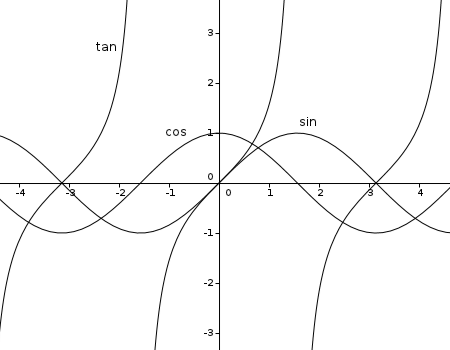
\includegraphics[scale=0.5]{trig1}
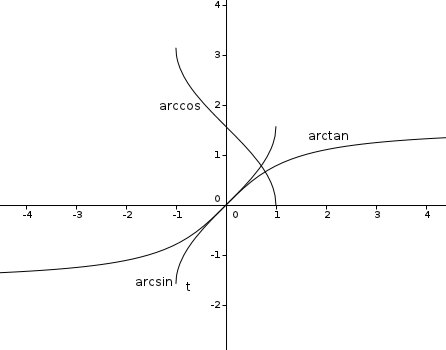
\includegraphics[scale=0.5]{trig2}
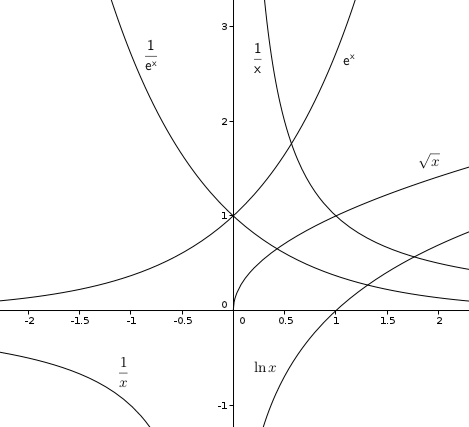
\includegraphics[scale=0.5]{umm}
\subsection{Sonstiges}
	$$
		\lim_{n \to \infty} \frac{e^{h_n} - 1}{h_n} = 1
	$$
	Plot von $\sin x \cos x$:\\
	http://www.wolframalpha.com/input/?i=plot+sin+x+cos+y

%
%
%
%
%
%
%
%
%
%
% end!
\end{document}

